% All contribution chapters should follow a similar structure, with a
% mini-introduction and overview at the beginning and a conclusion at the
% end bookmarking a structured presentation of the contribution. This can be
% largely based on your publications.

\chapter{Structure of the Agent-Based Model}\label{chap:contrib1}



The agent-based model of the 2D biofilm monolayer is structured around three main mechanisms. The first mechanism involves the release and diffusion of signaling molecules throughout a two-dimensional grid that covers the entire area of the biofilm. The second mechanism consists of biological functions that occur within individual bacterial cells. These functions include cell growth, reproduction, differentiation of phenotypes, and the detection of chemical signals in the environment. The third mechanism focuses on the physical volume exclusion interactions that occur between cells. These three main mechanisms are implemented in a continuous cycle, sequentially, as shown in Figure 3.1.

\begin{figure}[h]
    \centering
    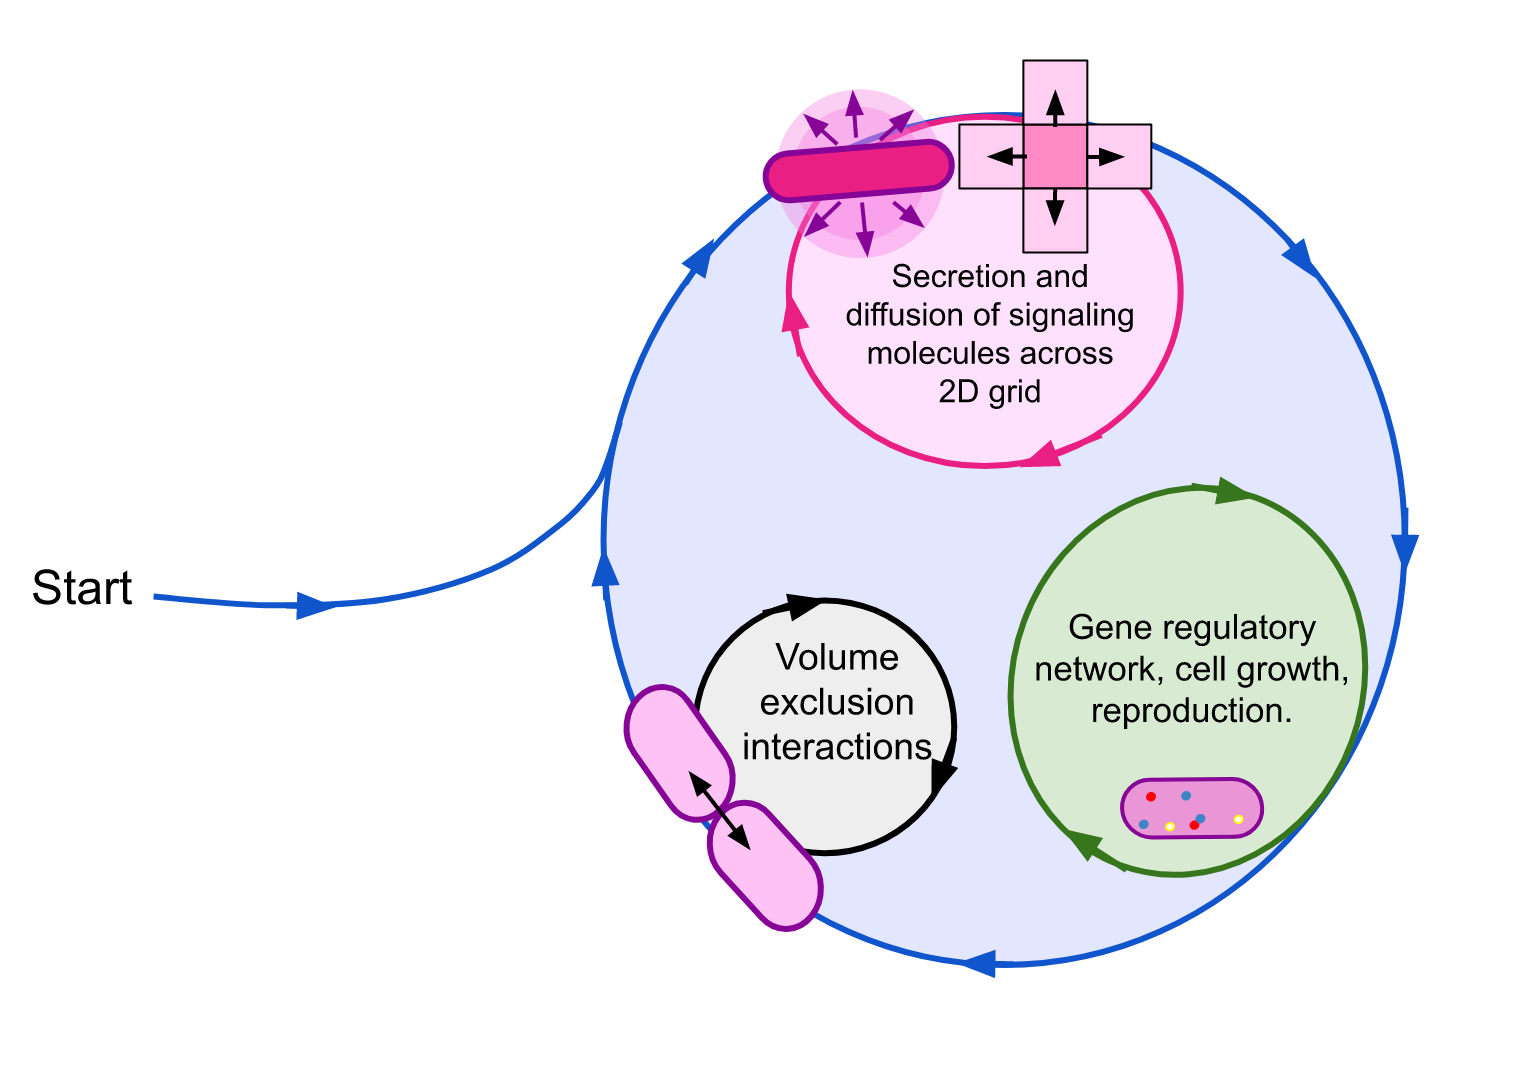
\includegraphics[width=1\textwidth]{cirkl}
    \caption{\footnotesize \textbf{Simulation steps.} The simulation begins with specific initial conditions, such as the starting number of cells, initial phenotypes, initial positions, and initial concentrations of regulatory proteins in the cytoplasm, among others. Then, the simulation runs the main simulation loop, which is subdivided into smaller loops corresponding to the secretion and diffusion of signaling molecules (in pink), biological functions (in green), and volume exclusion interactions (in gray).}

\end{figure} 

\begin{figure}[h]
    \centering
    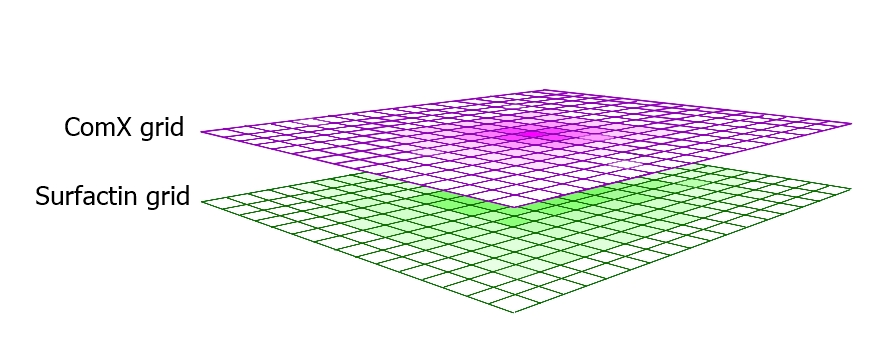
\includegraphics[width=1\textwidth]{grid}
    \caption{\footnotesize \textbf{Grids for numerical simulation of diffusion of signaling molecules}. There is a grid for each relevant substance in the model. The numerical simulation of diffusion runs independently on each separate grid.}

\end{figure}

\section{Secretion and diffusion of signaling molecules on the 2D grid}\label{sec:contrib1:theme1}

The model represents the extracellular environment as a square grid composed of 2025 pixels (45 by 45 pixels), where signaling molecules diffuse. This grid is useful for solving the diffusion equation using the finite difference method. Each pixel represents an area of 10 µm x 10 µm. The columns and rows of the grid define the coordinates of the two-dimensional space. In this space, each pixel represents the concentration of a signaling molecule at a specific coordinate. The model aims to simulate the diffusion process of two substances: ComX and surfactin. It employs separate, independent grids for each substance, as illustrated in Figure 3.2.

Every bacterium has the ability to interact with the pixel grid, either by secreting a substance onto the grid or by sensing it. In each iteration of the simulation, bacteria release a small amount of signaling molecules into the nearest pixel. Immediately after this release, the simulation performs a diffusion step to smooth out the initial peak resulting from the release of the signaling molecules. The detailed mathematical aspects of the diffusion simulation are presented in Chapter 4.




\section{Biological functions}\label{sec:contrib1:theme1:A}

The bacteria have been programmed to perform the following biological functions:

\subsection{Motion} This function introduces a small random force and torque to each individual bacterium, simulating Brownian motion. The random motion and growth of bacteria often result in bacterial cells overlapping in volume. A volume exclusion mechanism, which will be explained later, resolves this overlap.

\subsection{Growth} This function multiplies the length of each individual bacterium by a specific scaling factor greater than 1. To prevent large groups of bacteria from duplicating simultaneously, the growth rate and reproduction length are varied throughout the simulation by adding a small random value to these parameters for each individual bacterium. In this way, we prevent synchronized reproduction.


\begin{figure}[h]
    \centering
    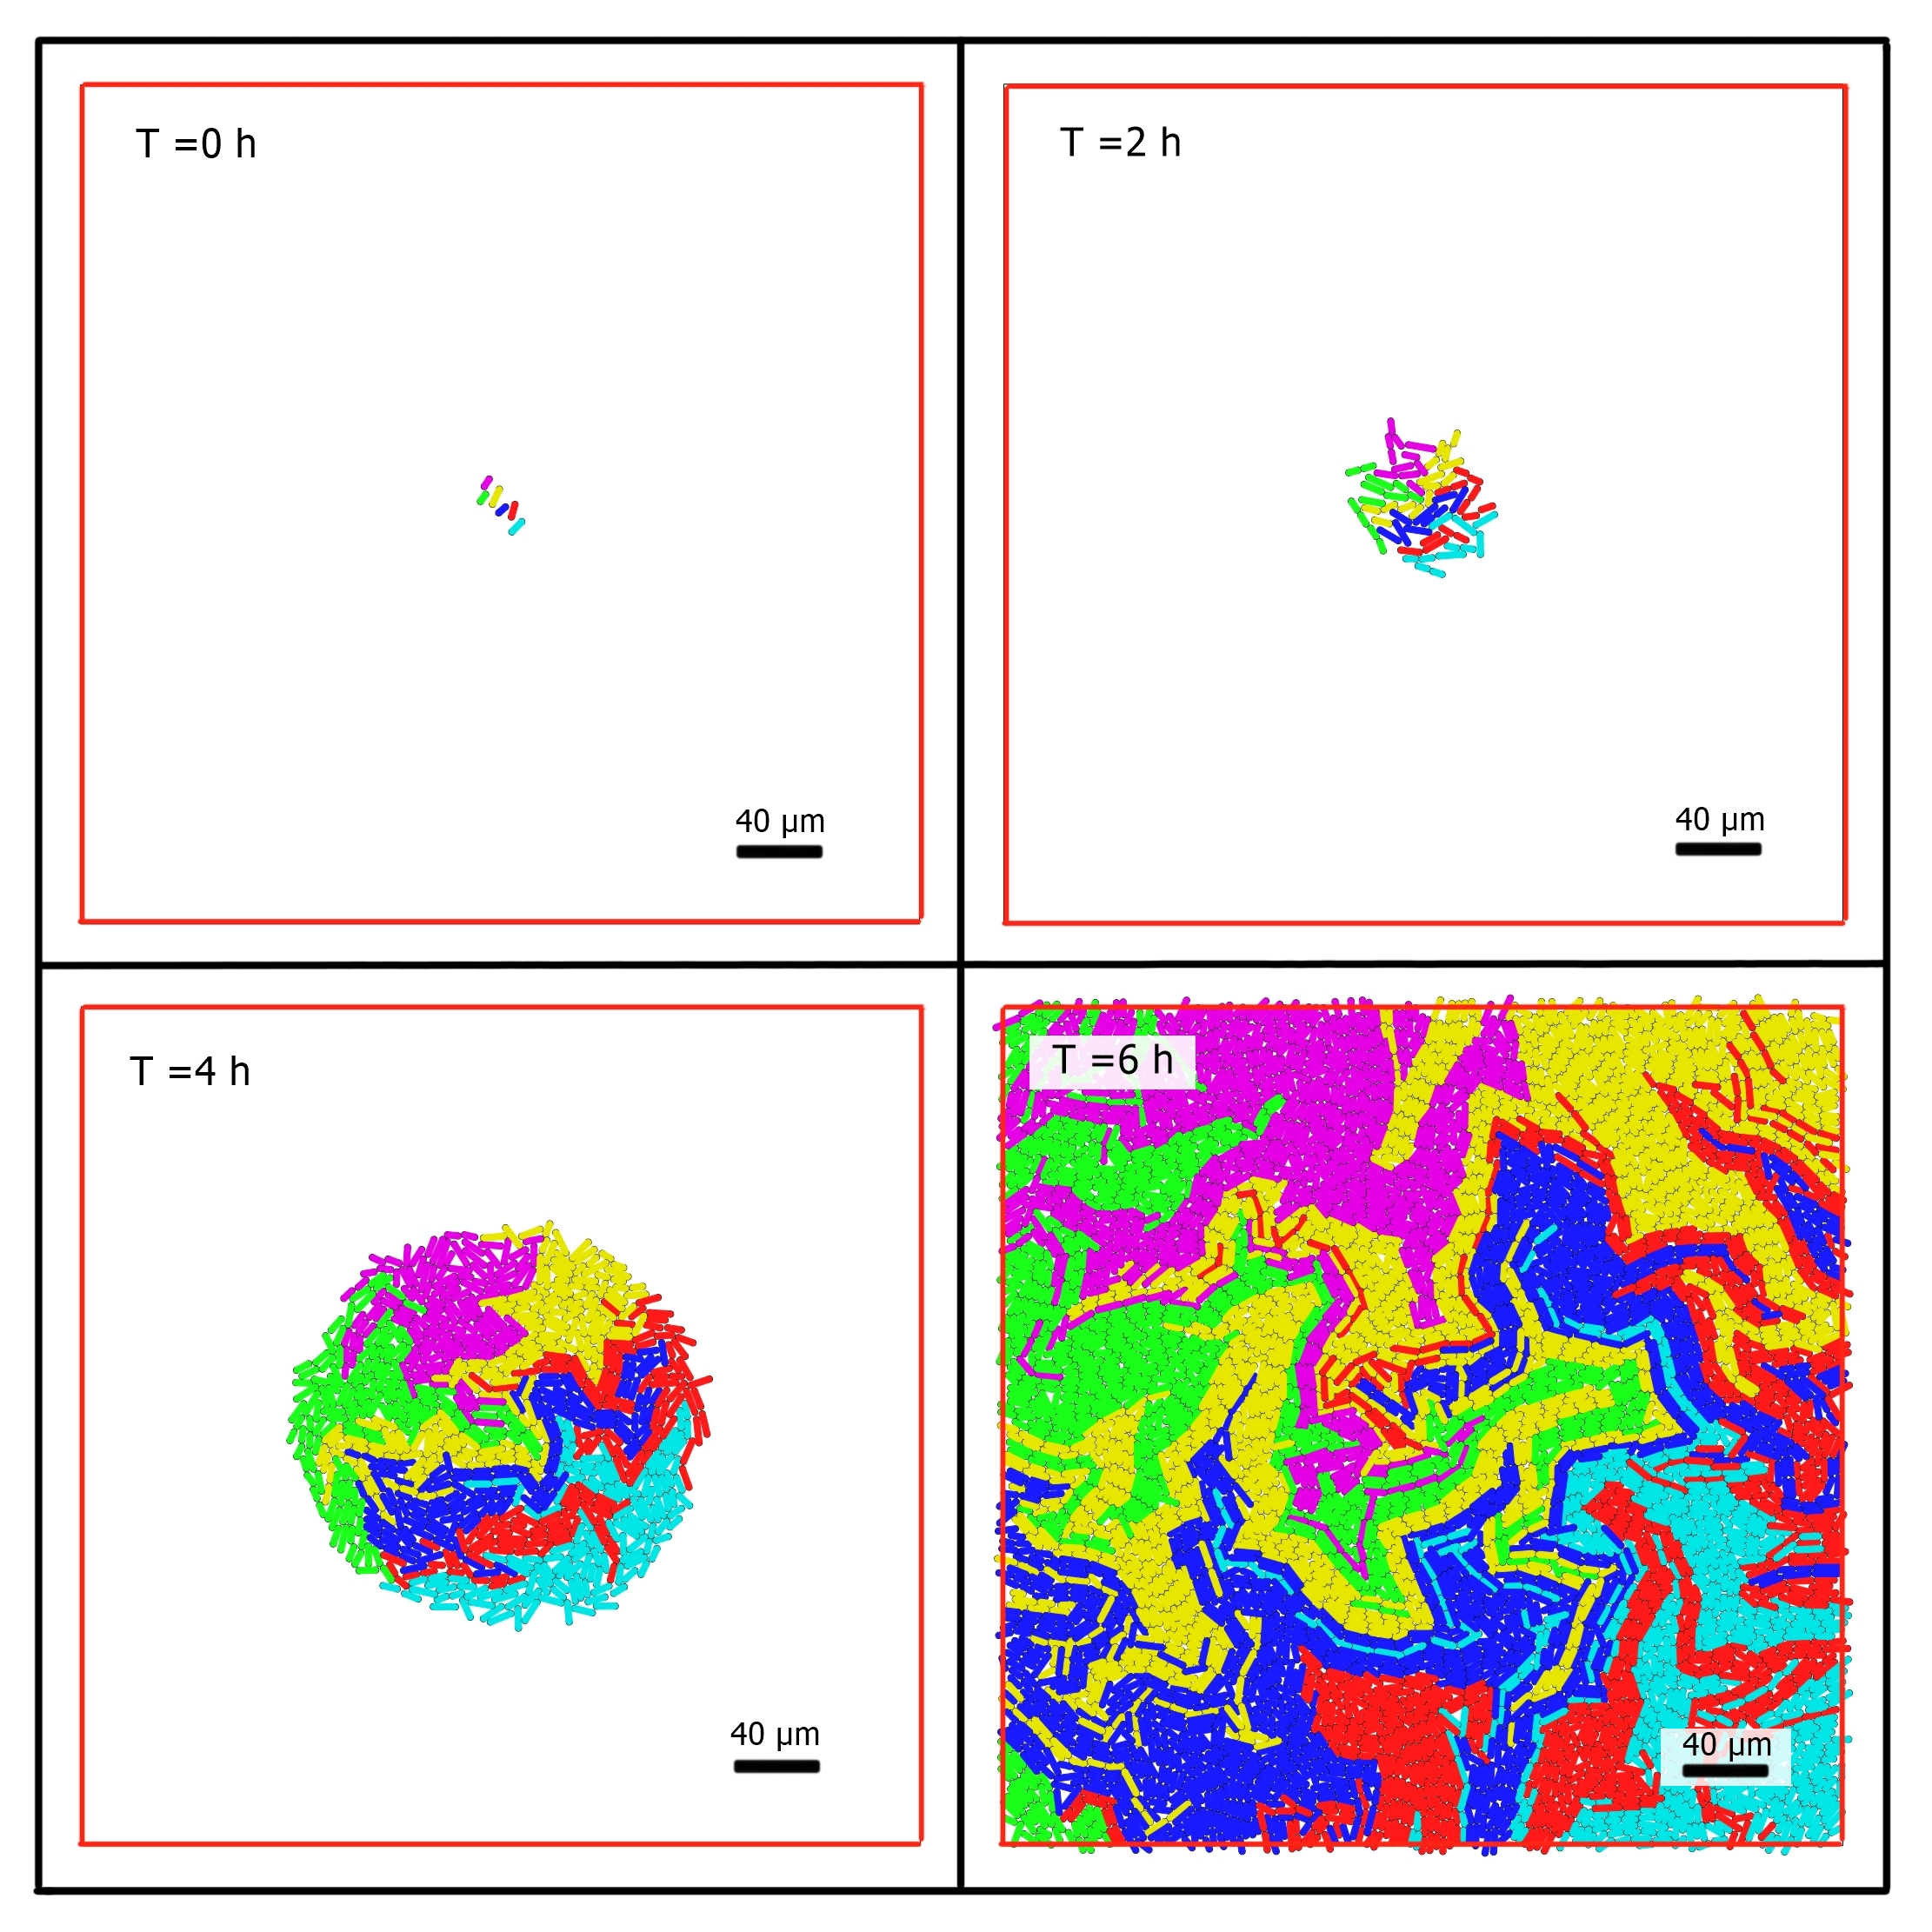
\includegraphics[width=0.9\textwidth]{New_engine2.jpg}
    \caption{\footnotesize \textbf{Demonstration of cell growth, reproduction, and inheritance.} The top-left corner shows six bacteria at the initial time step. Each of the six colors represent a distinct cell lineage. The top-right, bottom-left, and bottom-right panels show the color-coded offspring of the initial bacteria after 2, 4, and 6 hours, respectively. The red square represents the simulation area, which measures 0.16 mm\(^2\), where the bacteria are allowed to exist. If the bacteria escape from this area, they will be removed from the simulation}
\end{figure}
\subsection{Reproduction and Inheritance} When a bacterium's length reaches a certain threshold for reproduction, this function generates a new offspring bacterium adjacent to the parent bacterium. Some properties of this offspring bacterium, such as the cytoplasmic concentration of regulatory proteins, are inherited from the parent, while others, such as the threshold for reproduction length and sensitivity to signaling molecules, are randomly determined at birth. The ability to pass on traits from parents to their offspring allows us to visually track the offspring of each bacterium by assigning a color to the bacterium as an inheritable characteristic, as shown in Figure 3.3.


\subsection{Gene Regulatory Network} This function performs one iteration of the system of differential equations that represents the Gene Regulatory Network described in Section 2.4.3. It models the changing cytoplasmic protein concentrations of SinR, SlrR, and SinI within each individual bacterium. The fact that the network is simulated independently within each bacterium's cytoplasm means that at any given simulation step with $N$ bacteria, there are $N$ independent instances of this system of differential equations being solved simultaneously and decoupled from each other.

\subsection{Phenotype Differentiation} This function determines whether the conditions are suitable for gene expression or phenotype transition. For instance, if the concentration of ComX exceeds a certain stochastic threshold, the bacteria will transition into the surfactin-producing phenotype. If the internal concentration of the regulatory protein SinR falls below a certain stochastic threshold, the bacteria will transition into the phenotype that produces the extracellular matrix.

In this model, each bacterial cell has a unique sensitivity threshold to the concentration of extracellular ComX and cytoplasmic SinR. The sensitivity to ComX is a uniformly distributed random variable between 50 and 150 Arbitrary Units (AU), and it remains constant over time for individual bacteria. This means that, on average, half of the undifferentiated cells will transition to the surfactin-producing phenotype once they detect an extracellular concentration of ComX of 100 (AU) or higher. According to this model, sensitivity to ComX is a population trait that is not inherited from the parent bacteria. Instead, it is randomly determined at the moment of birth. The stochasticity of this trait within the population is the reason why it may appear that certain bacteria are sensitive to ComX, while others are not. In this way, a sufficiently high concentration of ComX will trigger any undifferentiated bacteria to become surfactin-producing bacteria. However, for a few bacteria, the stochastic threshold is so high that it will never be reached under normal conditions of cell density, ComX diffusion constant, and ComX production rate.

In the pathway involving surfactin, Spo0A, and KinC, we had to make some assumptions to simplify the model. We defined the intracellular concentration of Spo0A to be a linear function of the extracellular concentration of surfactin. This decision was based on the rough estimation of the presumed cytoplasmic concentration of Spo0A and the suggested molecular mechanism of Spo0A activation by surfactin through KinC phosphorylation (as illustrated in Figure 2.3). However, the interaction between these molecules could be further explored to develop a more comprehensive and detailed model.

Regarding the system of differential equations described in Section 2.4.3, we defined the SinR sensitivity threshold as a uniformly distributed random variable ranging from 47.5 to 52.5 nM. This means that, on average, half of the undifferentiated cells will transition to the matrix-producing phenotype once they detect a concentration of SinR that is 50 nM or lower.

\section{Volume exclusion interactions}\label{sec:contrib1:theme2}

The open-source TypeScript library, Box2d.ts, handles volume exclusion interactions, motion, and bacteria positions in the simulation. This 2D physics library helps to create animations that simulate the movements and interactions of rigid 2D objects. It offers tools for simulating physical phenomena like gravity, collisions, air resistance, and other forces that are specific to 2D graphics.{\footnotesize\cite{Catto2023}} For more information, please refer to section 7.1.

Without the volume exclusion mechanism, the growth and division of bacteria could result in overlapping cell volumes. The volume exclusion mechanism ensures that cells are displaced during their growth and division, as shown in Figure 3.3.

Additionally, this library was utilized to control the maximum number of bacteria allowed to coexist simultaneously within the simulation area. This control mechanism is crucial because unregulated bacterial exponential growth would make the simulation unmanageable. To achieve population control, there is a designated area of 0.16 mm\(^2\) within the simulation where the bacteria are allowed to exist. If a bacterium is pushed outside this area by its growing siblings, it will be eliminated from the simulation. According to our simulations, the maximum allowable amount of bacteria in this 0.16 mm\(^2\) area is approximately 5200 cells.


\section{Conclusion}\label{sec:contrib1:conclusion}

% Here we will summarize the contribution, and describe a logic transition to the next chapter.

%In this chapter, we presented the overall structure of the agent-based model of the 2D biofilm monolayer, which consists of three main mechanisms: the secretion and diffusion of signaling molecules on the 2D grid, biological functions like growth and reproduction, and volume exclusion interactions. In the following chapter, we will discuss the mathematical principles involved in simulating diffusion on a 2D grid. Additionally, we will also present the calculations used to determine the time scales at which several processes occur in the model.

% Let's make it better. We can do it!

In this chapter, we have presented the basic mechanisms of the agent-based model for the two-dimensional biofilm monolayer. The model consists of three main mechanisms: the secretion and diffusion of signaling molecules on a two-dimensional grid, biological functions such as growth and reproduction, and volume exclusion interactions. In the upcoming chapter, we will discuss the mathematical principles involved in simulating diffusion on a two-dimensional grid. Additionally, we will also present the calculations used to determine the time scales at which several processes occur in the model.
